\documentclass[]{report}

\usepackage{import}

\import{../}{settings.tex}

\title{Cours de probabilité pour l'agrégation}

\author{Cours de Mathieu MERLE, transcrit par SADR TAHOURI Luca}
\date{}



\begin{document}

\maketitle
\tableofcontents

\chapter{Espaces mesurés}

\section{Introduction}

La théorie de la mesure fournit un cadre mathématique commun pour
\begin{itemize}
    \item Notions classiques de mesure (distance, aire, volume) et les intégrales associées
    \item Formalisation et quantification d'expériences aléatoires.
          \begin{itemize}[label=$\hookrightarrow$]
              \item Expérience dont le résultat est imprévisible.
              \item Quantités moyennées
          \end{itemize}
\end{itemize}

\begin{ex}{}{}
    \begin{enumerate}
        \item "Temps" du vainqueur du $100m$ e.g. aux J.O.\\
              Ce qu'on peut mesurer dépend de la précision de l'appareil de mesure.\\
              Avec un chronomètre au 10e de seconde, $T$ étant le temps du vainqueur,
              \[\text{L'évènement } \cho{\left\{ T\le 10\right\}\text{ est mesurable}\\ \text{mais }\left\{10,24\le T\le 10,28\right\}\text{ ne l'est pas} }\]
        \item (Exo 2 du TD) Une contient $b$ boules bleues et $r$ boules rouges.\\
              Tirages uniformes, successifs, sans remise. Pour $k\ge 1$
              \[\Pa\left(\text{1er rouge soit tirée lors du $k$e tirage}\right)=\dfrac{b}{b+r}\dfrac{b-1}{b+r-1}\ldots \dfrac{b-k+2}{b+r-k+2}\dfrac{r}{b+r-k+1}\]
        \item mesure de l'aire cultivable d'un champ rectangulaire, au milieu duquel se trouve une mare
              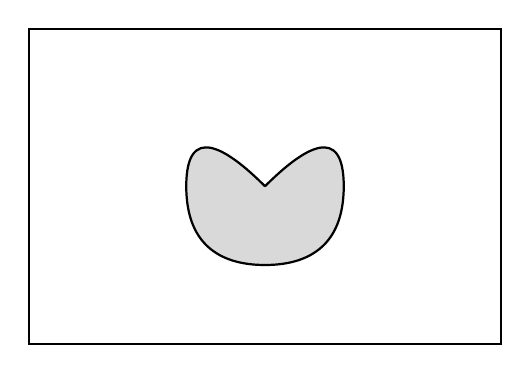
\begin{tikzpicture}
                  % Dessiner le rectangle
                  \draw[thick] (0,0) rectangle (6,4);

                  % Dessiner la mare au centre (forme plus organique et réaliste)
                  \draw[thick, fill=gray!30] (3,2) .. controls (2.5,2.5) and (2,2.8) .. (2,2)
                  .. controls (2,1.2) and (2.5,1) .. (3,1)
                  .. controls (3.5,1) and (4,1.2) .. (4,2)
                  .. controls (4,2.8) and (3.5,2.5) .. (3,2);
              \end{tikzpicture}
    \end{enumerate}
\end{ex}

\section{Tribus, mesures, exemples fondamentaux, caractérisation d'une mesure de probabilité}

$\Omega$ un ensemble quelconque, qu'on appelle "Univers"

\begin{df}{Tribu et espace mesurable}{}
    $\Fr\subset \Par(\Omega)$ est une tribu sur $\Omega$ si
    \begin{enumerate}[label=\roman*]
        \item $\Omega\in \Fr$
        \item $A\in \Fr\implies A^C\in \Fr$
        \item $(A_n)\subset \Fr\implies \bigcup_{\nN} A_n\in \Fr$
    \end{enumerate}
    On appelle $(\Omega,\Fr)$ un espace mesurable
\end{df}

\begin{prop}{}{}
    \begin{enumerate}[label=\alph*]
        \item $\emptyset\in \Fr$
        \item $A_1,\ldots,A_n\in \Fr$ alors $\bigcup_{i\in \llbracket 1,n\rrbracket} A_i \in \Fr, \bigcap_{i\in \llbracket 1,n \rrbracket} A_i \in \Fr$
        \item $A,B\in \Fr, B\wt A\in \Fr, A \qquad A\triangle B=(A\cup B)\wt (A\cap B)\in \Fr$
        \item $(A_n)\in \Fr^\N,\limsup A_n=\bigcap_n \bigcup_{p\ge n}A_p\in \Fr,\liminf A_n=\bigcup_n \bigcap_{p\ge n} A_p$
    \end{enumerate}
\end{prop}

\begin{df}{Mesure positive, espace mesuré, mesure $\sigma$-finie, mesure de probabilité, espace probabilisé}{}
    $\mu$ mesure positive sur $(\Omega,\Fr)$ si $\funto{\mu}{ \Fr}{\R_+ \cup \{+\infty\}}$ tq
    \begin{enumerate}[label=\roman*]
        \item $\mu (\emptyset)=0$
        \item $(A_n)_\nN\in \Fr^\N$ 2 à 2 disjoints,
              \[ \mu \left( \bigcup_\nN A_n \right)=\sum_\nN \mu(A_n)\]
    \end{enumerate}
    On dit que $(\Omega,\Fr,\mu)$ est un espace mesuré
    \begin{itemize}
        \item Si $\exists (\Omega_n)\nearrow$ tq $\bigcup_\nN \Omega_n=\Omega$, $\mu(\Omega_n)<+\infty,\forall n\in \N$, on dit que $\mu $ est $\sigma$-finie.
        \item Si $\mu(\Omega)=1$, on dit que $\mu$ est une probabilité, et alors $(\Omega,\Fr,\mu)$ est un espace probabilisé.
    \end{itemize}
\end{df}

\begin{prop}{}{}
    \begin{enumerate}[label=\alph*]
        \item $A_1,\ldots,A_n\in \Fr$, 2 à 2 disjoints
              \[ \mu\left( \bigcup_{k=1}^n A_k\right)= \sum_{i=1}^n \mu (A_i)\]
        \item \[\forall A,B\in \Fr,\mu(a)+\mu(B)=\mu(A\cup B)+ \mu(A\cap B)\]
        \item \[A\subset B, A,B\in \Fr, \mu(A)\le \mu(B)\]
              et si $\mu(A)<+\infty, \mu(B\wt A)=\mu(B)-\mu (A)$\\
              $(A_n)\in \Fr^\N,\mu(\bigcup_\nN A_n)\le \sum_{\nN} \mu(A_n)$
        \item $(A_n)\in \Fr^\N \nearrow,\mu\left(\bigcup A_n\right)=\lim \mu(A_n)$\\
              $(A_n)\in \Fr^\N \searrow,\mu\left(\bigcap A_n\right)=\lim \mu(A_n)$
    \end{enumerate}
\end{prop}

\begin{prop}{}{}
    \begin{enumerate}[label=\alph*]
        \item Si $\forall i\in I,\Fr_i$ est une tribu sur $\Omega$, alors $\bigcap_{i\in I}\Fr_i$ est une tribu sur $\Omega$
        \item $\Ar\subset \Pr(\Omega)$, on note $\sigma(A)$ et on appelle tribu engendrée par $\Ar$,
              \[\sigma(A):=\bigcap_{\substack{\Fr \text{ tribu sur $\Omega$}\\  \Ar\subset \Fr}} \Fr\]
              L'intersection est non vide car $\Par(\Omega)$ est une tribu sur $\Omega$ et $\sigma(A)$ est la plus petite tribu sur $\Omega$ contenant $\Ar$
    \end{enumerate}
\end{prop}

\begin{df}{Tribu des Boréliens}{}
    Si $\Omega$ est un espace topologique, $\Br(\Omega)$ la tribu des boréliens de $\Omega$ est
    \[\Br(\Omega)=\sigma\left(\left\{\text{ouverts de $\Omega$}\right\}\right)\]
\end{df}

\begin{df}{Tribu produit}{}
    $(E,\Ar),(\Fr,\Br)$ espaces mesurables
    \[\Ar\otimes \Br := \sigma \left(\left\{A\times B,A\in \Ar,B\in \Br\right\}\right)\]
    est la tribu produit
\end{df}

\begin{prop}{}{}
    \[\Br(\R)^{\otimes d}=\Br (\R^d)\]
\end{prop}

\begin{df}{Mesure produit}{}
    $(E,\Ar,\mu),(F,\Br,\nu)$ espaces mesurés, alors
    \[\funto{\mu \otimes \nu}{\Ar\otimes \Br}{\R_+\cup \{+\infty\}}\]
    l'unique mesure telle que $\forall A\in \Ar,B\in \Br$
    \[\mu\otimes \nu(A\times B)= \mu(A)\times \nu (B)\]
\end{df}

\begin{tm}{Existence et unicité de la mesure de Lebesgue}{}
    Il existe une unique mesure sur $(\R,\Br(\R))$, notée $\lambda$ et appelée mesure de Lebesgue telle que
    \[\lambda\left(]a,b[\right)=b-a,\forall (a,b)\in \R^2\]
    Il existe une unique mesure $\lambda_d$ sur $\left(\R^d,\Br(\R^d)\right)$ telle que
    \[\lambda\left(\produit{i=1}{d} ]a_i,b_i[\right)=\produit{i=1}{d}(b_i-a_i)\]
    \begin{itemize}
        \item De plus, $\lambda_d=\lambda^{\otimes d}$
        \item $\lambda_d$ est aussi l'unique mesure sur $\left(\R^d,\Br(\R^d)\right)$ invariante par translation telle que $\lambda_d\left([0,1]^d\right)=1$
    \end{itemize}
\end{tm}

\begin{prop}{}{}
    $\funto{f}{\Omega}{E}$ et $\Gr$ tribu sur $E$. On note
    \[f^{-1}(\Gr):=\left\{f^{-1}(B),B\in \Gr\right\}\]
    C'est une tribu sur $\Omega$. On l'appelle la tribu "Image réciproque" de $\Gr$ par $f$.\\
    Si $\Fr$ est une tribu sur $\Omega$,
    \[f^{\to}(\Fr):=\left\{B,f^{-1}(B)\in \Fr\right\}\]
    C'est une tribu sur $E$. On l'appelle "tribu image directe" de $\Fr$ par $f$\\
    Si $(\Omega,\Fr,\mu)$ espace mesuré, on peut définir $\mu_f$ ou $\mu\circ f$ la mesure image de $\mu$ par $f$,
    \[\fundfto{\mu_f}{f^{\to}(\Fr)}{\R_+\cup \{+\infty\}}{B}{\mu(f^{-1}(B))}\]
\end{prop}

\subsection{Applications mesurables: Rappels et remarques}

\begin{df}{Applications mesurables}{}
    $\funto{f}{E}{F}$ est dite mesurable de $(E,\Er)$ vers $(F,\Fr)$ si
    \[\forall B\in \Fr, f^{-1}(B)\in \Er\]
    En pratique, on aura souvent $F=\R$ ou $\R^d$
\end{df}

\begin{prop}{Applications mesurables}{}
    $\funto{f}{E}{F}$ est mesurable de $(E,\Er)$ vers $(F,\Fr)$ si pour $\Cr$ telle que $\sigma(\Cr)=\Fr$,
    \[\forall C\in \Cr, f^{-1}(C)\in \Er\]
\end{prop}

\begin{dfprop}{Mesure image}{}
    Si $(E,\Er,\mu)$ espace mesuré, $\mu_f$ (ou $f\circ \mu$) définit une mesure sur $(F,\Fr)$
    \[\forall B\in \Fr, \mu_f(B)=\mu\left(f^{-1}(B)\right)\]
\end{dfprop}

\begin{lm}{Lemme d'unicité de la mesure}{}
    Soient $(\mu_1,\mu_2)$ deux mesures sur $\Omega,\Fr$ telles que
    \begin{enumerate}
        \item $\exists (\Omega_n)\nearrow \Omega$ et $\mu_1(\Omega_n)=\mu_2(\Omega_n)<+\infty$
        \item $\exists \Cr$ stable par intersections finies telle que $\sigma(C)=\Fr$ et $\forall C\in \Cr,\mu_1(C)=\mu_2(\Cr)$
    \end{enumerate}
    Alors $\mu_1=\mu_2$
\end{lm}

\begin{df}{Classe monotone}{}
    $\Mr \subset \Pr(\Omega)$ est une classe monotone sur $\Omega$ si:
    \begin{enumerate}[label=\roman*]
        \item $\Omega \in \Mr$
        \item $A,B\in \Mr,A\subset B\implies B\wt A\in \Mr$
        \item $(A_n)_\nN\nearrow \in \Mr^\N\implies \bigcup_{\nN} A_n\in \Mr$
    \end{enumerate}
\end{df}

\begin{prop}{Intersection de classes monotones}{}
    Une intersection de classes monotones sur $\Omega$ est une classe monotone.
\end{prop}

\begin{lm}{Lemme des classes monotones}{}
    Soit $\Cr\subset \Pr(\Omega)$, stable par intersections finies, alors $\Mr(\Cr)=\sigma(\Cr)$
\end{lm}

\begin{proof}{Lemme des classes monotones}{}
    On veut montrer que $A,B\in \Mr(\Cr)\implies A\cap B\in \Mr(\Cr)$. Soit $A\in \Cr$,
    \[\Dr_A:=\{B\in \Mr(\Cr),A\cap B \in \Mr(\Cr)\}\]
    $\Dr_A$ est une classe montone et $\Cr\subset \Dr_A$ donc $\Dr_A=\Mr(\Cr)$. D'où
    \[\forall A\in \Cr,\forall B\in \Mr(\Cr),A\cap B\in \Mr(\Cr)\]
    Soit $A\in \Mr(\Cr),\Dr(A)$ classe monotone contient $\Cr$ par ce qui précède, donc $\Dr_A=\Mr(\Cr)$
\end{proof}

\begin{proof}{Lemme d'unicité de la mesure}{}
    Si $\mu_1,\mu_2$ deux mesures finies et $\mu_1(\Omega)=\mu_2(\Omega)$, $\forall C\in \Cr, \mu_1(C)=\mu_2(C)$.
    \[\Mr=\{B\in \Fr,\mu_1(B)=\mu_2(B)\}\]
    est une classe monotone qui contient $\Cr$ donc $\Mr= \Fr$ par le lemme d'unicité des classes monotones.\\
    On peut ensuite considérer $\mu_{1|\Omega_n},\mu_{2|\Omega_n}$ et appliquer ce qu'il y a juste avant.
\end{proof}

\begin{prop}{Conséquences du lemme d'unicité}{}
    \begin{enumerate}
        \item L'unicité de la mesure de Lebesgue sur $\R^n,\forall n\in \N^*$
        \item Avec la condition 1 dans le lemme d'unicité des mesures est inutile si $\mu_1$ et $\mu_2$ sont des mesures de probabilité
              \begin{enumerate}
                  \item $(A_k)_{k\in K}$ partition de $\Omega$ avec $K$ fini ou dénombrable.
                        \[\Fr=\sigma(A_k,k\in K)\]
                        \[\Cr=\{A_k,k\in K,\emptyset\}\]
                        Pour caractériser $\Pa$ sur $(\Omega,\Fr)$, il suffit de connaître $p_k=\Pa(A_k),k\in K$
                  \item Si $\Omega=\R,\Fr=\Br(\R),\Cr:=\{]-\infty,a],a\in \R\}$. Se donner
                        \[\fundfto{F}{\Cr}{[0,1]}{]-\infty,a]}{\Pa(]-\infty,a])}\]
              \end{enumerate}
        \item $\Omega=\{0,1\}^{\N^*}$ muni de la tribu cylindrique.
              \[\Fr=\sigma\left(\{\text{cylindres}\}\right)\]
              où un cylindre est un évènement qui ne dépend que d'un nombre fini de coordonnées.\\
              Le lemme d'unicité de la mesure permet d'affirmer que pouir caractériser $\Pa$ sur $(\Omega,\Fr)$, il suffit de se donner la mesure de chaque cylindre ou même de chaque cylindre élémentaire : $\forall n\in \N^*,\forall (\epsilon_1,\ldots,\epsilon_n)\in \{0,1\}^n$
    \end{enumerate}
\end{prop}

\section{Dénombrement: exemples formalisés de probabilités discrètes}

\subsection{Exemples d'espaces}

\begin{ex}{}{}
    \begin{enumerate}
        \item \[\{r,\text{tirage ordonné successif, sans remise, parmis $n$ objets}\}\]
              \[\updownarrow\]
              \[\{\text{Placement de $r$ boules numérotées dans $n$ cases numérotées, max $1$ boule par case}\}\]
              \[\updownarrow\]
              \[\{\funto{f}{\{1,\ldots,r\}}{\{1,\ldots,r\}}\text{ injective}\}\]
        \item \[\{r\text{ tirages ordonnés, avec remise parmis $n$ objets}\}\]
              \[\updownarrow\]
              \[\{\text{placements de $r$ boules numérotées dans $n$ cases numérotées}\}\]
              \[\updownarrow\]
              \[\{\funto{f}{\{1,\ldots,r\}}{\{1,\ldots,n\}}\}\]
              Cardinal commun $n^r$
        \item \[\{\text{tirage simultané de $r$ objets parmis $n$}\}\]
              \[\updownarrow\]
              \[\{\text{cases occupées lors du placement de $r$ boules (indistingables) dans $n$ cases, max $1$ boule par case}\}\]
              \[\updownarrow\]
              \[\{Im f,\funto{f}{\{1,\ldots,n\}}{\{1,\ldots,n\}},\text{ injective}\}\]
    \end{enumerate}
\end{ex}

\subsection{Exemples classiques}

VOIR PHOTOS 30/09

\section{Probas conditionnelles: cadre discret}

Soit $(\Omega,\Fr,\Pa)$ espace probabilisé.

\subsection{Définitions}

\begin{df}{Conditionnement et probabilité conditionnelle}{}
    Soit $B\in \Fr,$ tq $\Pa(B)>0$, on définit le conditionnement
    \[\Pa(A|B)=\frac{\Pa(A\cap B)}{\Pa( B)},\forall A\in \Fr\]
    On appelle probabilité conditionnelle sachant $B$, on note $\Pa_B$ la proba:
    \[\fundfto{\Pa_B}{\Fr}{[0,1]}{A}{\Pa(A|B)}\]
\end{df}

\begin{tm}{Conditionnements successifs}{}
    Soit $(A_1,\ldots,A_n)\in \Fr^n, \Pa(A_1\cap \ldots \cap A_{n-1})>0$, alors
    \[\Pa(A_1\cap \ldots\cap A_n)=\Pa(A_1)\Pa(A_2|A_1)\Pa(A_3|A_1\cap A_2)\ldots \Pa(A_n)| A_1\cap A_2\cap \ldots \cap A_{n-1}\]
\end{tm}

\subsection{Probabilité totale, Bayes}

\begin{tm}{Probabilités totales}{}
    $(\Omega_j)_{j\in J}$ avec $J$ fini ou dénombrable partition de $\Omega$, $\Omega_j \in \Fr,\Pa(\Omega_j)>0,\forall j\in J$. Alors
    \[\forall A\in \Fr, \Pa(A)=\sum_{j\in J} \Pa(A\cap \Omega_j)=\sum_{j\in J} \Pa(A|\Omega_j)\Pa(\Omega_j)\]
\end{tm}

\begin{proof}{Probabilités totales}{}
    Exercice (A FAIRE)
\end{proof}

\begin{tm}{Bayes}{}
    Pour $A\in \Fr, \Pa(A)>0$,
    \[\Pa(\Omega_{j_0})=\frac{\Pa(A|\Omega_{j_0})\Pa(\Omega_{j_0})}{\sum_{j\in J} \Pa(A|\Omega_j)\Pa(\Omega_j)}\]
\end{tm}

\begin{proof}{Bayes}{}
    Exercice (A FAIRE)
\end{proof}

\section{Indépendance d'évènements, de tribus, Borel-Cantelli, loi du $0-1$}

\begin{df}{Indépendances de deux évènements}{}
    Soit $(A,\Fr,\Pa)$ espace probabilisé. Soient $A$ et $B$ deux éléments de $\Fr$. On dit que $A$ et $B$ sont indépendants si
    \[\Pa(A\cap B)=\Pa(A)\Pa(B)\]
\end{df}

\begin{df}{Indépendance d'une famille d'évènements}{}
    Soient $(A_i)_{i\in I}$ famille d'éléments de $\Fr$. On dit que les $A_i$ sont indépendants si
    \[\forall J\subset I,I\text{ fini}, \Pa\left(\bigcap_{j\in J}A_j\right)=\prod_{j\in J} \Pa(A_j)\]
\end{df}

\begin{prop}{}{}
    L'indépendance implique l'indépendance deux à deux.\\
    De manière plus générale, si $K\subset I$, si $(A_i)_{i\in I}$ est indépendante alors $(A_k)_{k\in K}$ aussi
\end{prop}

\begin{tm}{Indépendance d'une famille finie}{}
    La famille finie d'événements $(A_i)_{1\le i\le n}$ est indépendante \ssi
    \[\forall B_i\in \{\emptyset,\Omega,A_i,A_i^C\},1\le i \le n, \quad \Pa\left(\bigcap_{i=1}^n B_i\right) \prod_{i=1}^{n}\Pa(B_i)\]
\end{tm}

\begin{lm}{Indépendance du complémentaire}{}
    Si $(A_1,\ldots,A_n)$ est indépendante, alors $(A_1^C,A_2,\ldots,A_n)$ l'est également
\end{lm}

\begin{proof}{Indépendance du complémentaire}{}
    A VOIR
\end{proof}

\begin{proof}{Indépendance d'une famille finie}{}
    A VOIR
\end{proof}

\begin{df}{Indépendance de tribus}{}
    A voir
\end{df}

\begin{tm}{Indépendances d'un nombre dénombrable de tribus}{}
    A voir    
\end{tm}

\begin{tm}{}{}
    Soient $\Cr\subset \Fr,\Dr\subset \Fr$ stables par intersections finies. Si
    \[\forall A\in \Cr,\forall B\in \Dr,\quad \Pa(A\cap B)=\Pa(A)\Pa(B)\]
    Alors les tribus $\sigma(\Cr)$ et $\sigma(\Dr)$ sont indépendantes
\end{tm}

\begin{proof}{}{}
    Soit $A\in \Cr,\Mr_A=\{B\in \sigma (\Dr), \Pa(A\cap B)=\Pa(A)\Pa(B)\}$ est une classe monotone qui contient $\Fr$ donc par le lemme des classes monotones c'est $\sigma(\Dr)$.\\
    Soit alors $B\in \sigma(\Dr),\Mr_B=\{A\in \sigma(\Cr),\Pa(A\cap B)=\Pa(A)\Pa(B)\}$ est une classe monotone, par ce qui précède elle contient $\Cr$ et par le lemme des classes monotones, $\sigma(\Cr)$
\end{proof}

Le théorème précédent se généralise aisément à une inte

\begin{tm}{}{}
    On suppose que les $\{\Fr_i,i\in I\}$ sont des tribus indépendantes, et que $K_1$ et $K_2$ sont tels que $K_1\cup K_2=I,K_1\cap K_2=\emptyset$. Alors $\Gr_1=\sigma\left(\bigcup_{k\in K_1}\Fr_k\right)$ et $\Gr_2=\sigma\left(\bigcup_{k\in K_2}\Fr_k\right)$ sont indépendantes.
\end{tm}

\begin{proof}{}{}
    \[C_1:=\{\bigcap_{j\in J} A_j,J\text{ fini},J\subset K_1,A_j\in \Fr_j,j\in J\}\]
    est stable par intersections finies et engendre $\Gr_1$
    \[C_2:=\{\bigcap_{j\in J} A_j,J\text{ fini},J\subset K_2,A_j\in \Fr_j,j\in J\}\]
    est stable par intersections finies et engendre $\Gr_2$. On conclut grâce au théorème précédent.
\end{proof}

On peut généraliser à une partition quelconque

\begin{tm}{}{}
    On suppose que les $\{\Fr_i,i\in I\}$ sont des tribus indépendantes et que $\{I_k,k\in K\}$ forme une partition quelconque de $I$. Alors les $\left(\Gr_k:=\sigma\left(\bigcup_{k\in I_k} \Fr_k\right),k\in K\right)$ sont indépendantes.
\end{tm}

\begin{lm}{Borel-Cantelli}{}
    Soient $\{A_n,n\in \N\}$ une famille d'événements tels que $\sum_{n\in \N}\Pa(A_n)<+\infty$, alors
    \[\Pa(\limsup A_n)=0\]
    Soient $\{A_n,n\in \N\}$ une famille d'événements indépendants, tels que $\sum_\nN\Pa(A_n)=+\infty$. Alors $\Pa(\limsup A_n)=1$
\end{lm}

\begin{proof}{Borel-Cantelli}{}
    Pour la première partie: $\Ea(\sum \1_{A_n})<+\infty$ implique que presque sûrement $\sum \1_{A_n}<+\infty$ et donc que p.s. $\limsup \1_{A_n}=0$\\
    Il s'agit de montrer que pour tout $p\in \N,\bigcap_{n\ge p} A_n^C$ est négligeable. Par indépendance, $\Pa\left(\bigcap_{n\ge p}A_n^C\right)=\prod_{n\ge p}(1-\Pa(A_n))$. Si par l'absurde, le membre de gauche est strictement positif, aucun des $A_n^C,n\ge p$ n'est pas négligeable et
    \[\ln \left(\Pa\left(\bigcap_{n\in\N}A_n^C\right)\right)=\sum_\nN \ln(1-\Pa(A_n))\]
    Comme pour tout $x\in [0,1[,\ln(1-x)\le -x$, on en déduit que
    \[\ln \left(\Pa\left(\bigcap_{n\in\N}A_n^C\right)\right)\le -\sum_{n\in \N}\Pa(A_n)=-\infty\]
    Contradiction
\end{proof}

\begin{tm}{Généralisation du second lemme de Borel-Cantelli}{}
    Soient $(A_n)$ une suite d'événements,
    \[N_n=\sum_{k=1}^{n}\1_{A_k},m_n=\sum_{k=1}^{n}\Pa(A_n)\]
    Si $\lim_{n\to \infty}m_n=+\infty,\lim_{n\to \infty} \frac{\Var(N_n)}{m_n^2}=0$, alors $\Pa(\limsup A_n)=1$
\end{tm}

\begin{proof}{}{}
    Soit $a>0$ fixé, et $n $ suffisamment grand pour que $m_n>a$,
    \[\Pa(N_n\le a)\le \Pa\left(|N_n-m_n|\ge m_n-a\right)\le \Ea\left[\frac{(N_n-m_n)^2}{(a-m_n)^2}\right]\]
    qui par hypothèse tend vers $0$, on conclut que pour tout $a>0$,
    \[\Pa\left(\sum_{k\ge n} \1_{A_k}\le a\right)=0\]
\end{proof}

\begin{df}{Tribu asymptotique}{}
    Soient $\{\Fr_n,n\in \N\}$ une famille de sous-tribus de $\Fr$, la tribu asymptotique est 
    \[\Fr_\infty:=\bigcap_\nN \sigma \left(\bigcup_{p\ge n} \Fr_p\right)\]
\end{df}

\begin{tm}{Loi du 0-1 de Kolmogorov}{}
    Si les tribus $\{\Fr_n,n\in \N\}$ sont indépendantes, alors $\Fr_\infty$ est triviale:
    \[\forall A\in \Fr_\infty,\Pa(A)\in \{0,1\}\]
\end{tm}

\begin{proof}{Loi du 0-1 de Kolmogorov}{}
    Soit $N\in \N$, par le théorème d'indépendance par paquets, les tribus
    \[\Gr_N:=\sigma\left(\bigcup_{n\in \N}\Fr_n\right)\quad \Hr_n:=\sigma\left(\bigcup_{n>N}\Fr_n\right)\] sont indépendantes et donc $\Gr_N$ et $\Fr_\infty$ sont indépendantes.\\
    Mais puisque ceci vaut pour tout $N$, $\Fr_\infty,\Fr,n\in \N$ restent indépendantes: la définition d'indépendance ne fait intervenir que des sous-ensembles d'indices finis.\\
    Quitte à regrouper par paquets, on déduit que $\Fr_\infty$ est indépendante de $\sigma\left(\bigcup_\nN \Fr_n\right)$ et on conclut que $\Fr_\infty$ est indépendante d'elle-même.
\end{proof}

Cela fonctionne aussi pour une famille quelconque (plus que dénombrable) de tribus.

\chapter{Variables aléatoires}

\section{Définitions,généralités}

\begin{df}{Variable aléatoire, loi de probabilité}{}
    Soit $(\Omega,\Fr,\Pa)$ un espace probabilisé, et $(E,\Er)$ un espace mesurable. $\funto{X}{\Omega}{E}$ est une variable aléatoire si $X$ est mesurable.\\
    La mesure de probabilité $\Pa_X$ définie par $\Pa_X(B)=\Pa(X^{-1}(B))$ est appelée la loi de $X$
\end{df}

\section{Espérance d'une variable aléatoire, rappels d'intégration}

\chapter{Convergence d'une suite de variables aléatoires et Théorèmes limites}

\chapter{Statistique}
\end{document}